\documentclass[twoside]{article}

\usepackage{lmodern}
\usepackage[T1]{fontenc}
\usepackage[spanish,activeacute]{babel}
\usepackage{mathtools}
\usepackage{graphicx}
\usepackage[inner=3.0cm,top=2.5cm,outer=2.0cm,bottom=2.5cm]{geometry}  
\usepackage{fancyhdr}
%\usepackage{hyperref}
%\usepackage[toc,xindy]{glossaries}

\pagenumbering{gobble}
\renewcommand{\baselinestretch}{1.5}
\setlength{\footskip}{43.0pt}

\title{\begin{center} 

\includegraphics[width=0.8\textwidth]{images/upc-logo.png} 
\end{center} 
\vspace{0.5cm} 
Proyecto Final de Carrera\\
INGENIER\'IA INDUSTRIAL \\
\vspace{0.5cm} 
\Huge{WifiBotPi} 
\vspace{0.5cm} \\
 Memoria}

\author{}
\date{} % void to avoid put current date
\pagestyle{fancy}

\fancyhead[LO,RE]{\title{WifiBotPiRos}}
\fancyhead[LE,RO]{\thepage}
\fancyfoot[LE,RO]{
\includegraphics[scale=0.5]{images/etseib-logo.png}}
\fancyfoot[C]{}
%\headrulewidth 0.4pt
%\footrulewidth 0 pt


\begin{document}
%\pagestyle{empty} 

\maketitle
\begin{center}
\large{$\begin{array}{ll}
\mbox{Autor:} & \mbox{Joan Guasch Iglesias} \\
\mbox{Director:} & \mbox{Manel Velasco Garcia} \\
\mbox{Convocatoria:} & \mbox{Fecha a presentar}
\end{array}$}\\ 
\vspace{2cm} 
\Large{Escuela T'ecnica Superior de Ingenier'ia Industrial de Barcelona}\\ \vspace{1cm}

\includegraphics[scale=1]{images/etseib-logo.png}
\end{center}
\thispagestyle{empty}
\newpage

\thispagestyle{empty}
\paragraph*{}
\newpage

%\thispagestyle{empty}
%\pagenumber{1}
\pagenumbering{arabic}
\fancyhead[LE,RO]{1}
\section*{Resumen}
Este proyecto consistir'a en el aprovechamiento de una plataforma rob'otica que corre el riesgo de quedarse obsoleta y rescatarla de su destino. Para ello se incorporar'an un conjunto de herramientas que simplificar'an el trabajo para futuros usuarios.
\newpage

\thispagestyle{empty}
\paragraph*{}
\newpage

\fancyhead[LE,RO]{3}

\tableofcontents
\setcounter{page}{1}
\addtocontents{toc}{~\hfill\textbf{P'agina}\par}
\addcontentsline{toc}{section}{Resumen}
%\setcounter{page}{3}
%\addcontentsline{toc}{section}{'Indice}
\newpage

%\pagenumbering{arabic}
\setcounter{page}{4}
\fancyhead[LE,RO]{\thepage}

\section{Glosario}
\newpage

\section{Prefacio}
\subsection{Motivaci'on}
\newpage

\section{Introducci'on}
\subsection{Historia}
\subsection{Estado del arte}
\subsection{Alcance}
\subsection{Objetivos}

\newpage
\section{Material de partida }

\subsection{WifiBot}
\textbf{Wifibot} es una plataforma rob'otica, desarrollada por la empresa francesa \textbf{Nexter Robotics}, dise'nada para poder navegar en m'ultiples escenarios gr'acias a su dise'no. Su sistema de tracci'on a las cuatro ruedas, dise'no reducido y bajo peso, le otorga una gran flexibilidad.

\subsubsection{Descripci'on}
Este proyecto partir'a del modelo \textbf{WifiBot 4G}, producido durante el periodo 2002--2006 y que incluye las siguientes caracter'isticas:

\begin{figure}[ht]
\centering
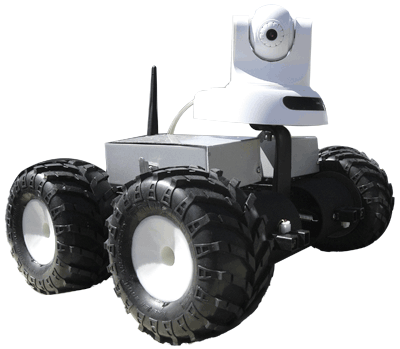
\includegraphics[scale=0.5]{images/Visuel_Wifibot_2.png} 
\caption{Wifi Bot 4G}
\label{fig:Wifi Bot 4G}
\end{figure}

\paragraph{Componentes}
\begin{itemize}
\item CPU:
	\begin{itemize}
	\item Procesador AMD Au1500
	\item 400MHz
	\item Mem'oria RAM de 64MB
	\item Mem'oria Flash de 32MB
	\end{itemize}
\item Interf'icies:
	\begin{itemize}
	\item 4x Ethernet 10/100
	\item 1x USB
	\item 1x I$^{2}$C
	\item 1x RS232
	\end{itemize}
\item WIFI:
	\begin{itemize}
	\item WiFi con est'andar 802.11a/b/g
	\item Modos Access Point, Bridge, Client y Router
	\item 1x Antena de 5dBi
	\end{itemize}
\item Sensores:
	\begin{itemize}
	\item 1x C'amara IP
	\item 2x Sensor IR de dist'ancia
	\item 2x Codificador de efecto Hall (Hall Encoder) 
	\item 2x DSPIC30F2010
	\item 1x Nivel de bater'ia
	\end{itemize}
\item Motores:
	\begin{itemize}
	\item 4x Motor de 7.2V
	\item Reductora $i=50:1$
	\item Par nominal 8.87Kg/cm
	\item Velocidad nominal 120Rpm
	\end{itemize}
\item Dimensiones:
	\begin{itemize}
	\item Longitud 28cm
	\item Anchura 30cm
	\item Altura 20cm
	\item Peso 4.5Kg
	\end{itemize}
\item Bater'ias:
	\begin{itemize}
	\item 9.6V NiMh (8 celdas)
	\item Capacidad 9500mAh
	\item Autonom'ia de 2 horas
	\end{itemize}
\end{itemize}

\paragraph{Estructura}\noindent

La estructura de la base est'a formada por dos secciones sim'etricas que llamaremos hemisferios izquierdo y derecho. Estas dos partes est'an unidas por una barra roscada que atraviesa transversalmente todo el robot, ofreciendo un eje de rotaci'on entre los dos elementos, cualidad que le otorga una mayor adaptaci'on a superf'icies irregulares.
%include image SolidWorks
%c'omo vemos en figura \ref{fig:Wifi Bot 4G}

\subsubsection{Estado Inicial}  
La plataforma de la que se dispon'ia en un principio carec'ia de cierta cualidades. La m'as destacable era la inestabilidad de la red WiFi, dicha conexi'on sufr'ia constantes ca'idas con lo que dificultaba enormemente su teleopraci'on. Su otro tal'on de Aquiles era su escasa documentaci'on disponible, al ser un producto que su fabricante da por descontinuado y al no disponer de una comunidad que lo mantenga, dicha base rob'otica provocaba quebraderos de cabeza para usuarios noveles. Finalmente, las bater'ias al haber completado su vida 'util, dispon'ian de una carga efectiva muy inferior a la inicial. 

En cambio, tanto la estructura, ruedas, motores y sensores se encontraban en mejores condiciones

\subsection{Raspberry Pi}
Raspberry Pi es un ordenador del tama'no de una tarjeta de cr'edito desarrolado en Reino Unido por la \textbf{Raspberry Pi Foundation}
\newpage

\section{Especificaciones}
Tal y como se ha definido anteriormente, el objetivo de este proyecto consiste en ofrecer una plataforma funcional para los futuros usuarios. Para definir esta ''funcionalidad'' se ha basado en el conocimiento aportado por antiguos usuarios, trabajadores en productos similares y en la experiencia propia. 

Las especificaciones se han clasificado seg'un su or'igen. Dependiendo de si son de car'acter \textbf{software}, \textbf{electr'onico} o \textbf{mec'anico}. Las especificaciones de car'acter inform'atico engloban aspectos como la interf'icie con el usuario, las herramientas de desarrollo (librer'ias, documentaci'on) y la disponibilidad a futuras modificaciones. Por contra, la electr'onica ha de evitar que el usuario se encuentre obligado a manipular el interior del robot, pero que en el caso de dicha situaci'on permita una soluci'on simple del problema. Adem'as, la electr'onica ha de incorporar un sistema que permita conocer estados del robot de manera sencilla. Finalmente, la mec'anica se encarga de incorporar las nuevas especificaciones en la plataforma, manteniendo el concepto inicial. Igual que en la electr'onica, en el caso de una futura manipulaci'on por parte del usuario, el dise'no ha de facilitar el acceso a cualquier ubicaci'on.

\subsection{Software}

\subsection{Electr'onica}

\subsection{Mec'anica}

\newpage
\section{Modificaciones}
Para la realizaci'on de este proyecto se deber'a trabajar en varios sectores 

\subsection{Electr'onica}
\newpage

\section{Conclusiones}
\newpage

\section{Agradecimientos}
\newpage

\section{Biografia}
\newpage

\section{Soporte inform'atico}

\end{document}